\chapter{Математическая модель движения безвинтового подводного робота с внутренними роторами в жидкости}\label{ch:ch2}

В данной главе представлены результаты разработки математической модели трехмерного движения безвинтового подводного робота с внутренними роторами в жидкости. Доказана управляемость системы при выполнении некоторых условий. Записаны значения коэффициентов, зависящих от формы и конструкции модели робота. На основании полученных уравнений движения проведено моделирование и получены траектории, движение по которым представляет собой базовые маневры. Для описания движения безвинтового подводного робота с внутренними роторами в жидкости разработана математическая модель, основанная на исследованиях В.В. Козлова и С.М. Рамоданова  в работах~\cite{Kozlov_Ramodanov_PMM_2001, Kozlov_Ramodanov_PAN_2002}. Модель подразумевает собой движение в идеальной жидкости в трехмерной постановке.

В записи уравнений все векторные величины записаны жирным шрифтом, скалярные величины --- нежирным шрифтом, матрицы обозначены прямыми жирными прописными буквами; скалярное произведение векторов $ \bbs{a} $ и $ \bbs{b} $ записывается как $ (\bbs{a}, \bbs{b}) $, а векторное произведение --- $ \bbs{a} \times \bbs{b} $.

\section{Уравнения движения}\label{sec:ch2/sec1}

Рассмотрим систему, состоящую из жесткой внешней оболочки, имеющей форму эллипсоида вращения, и трех внутренних роторов (рисунок \ref{rotors}). %Геометрический центр системы совпадает с центром сферической части оболочки.

\begin{figure}[th]
	\begin{center}
		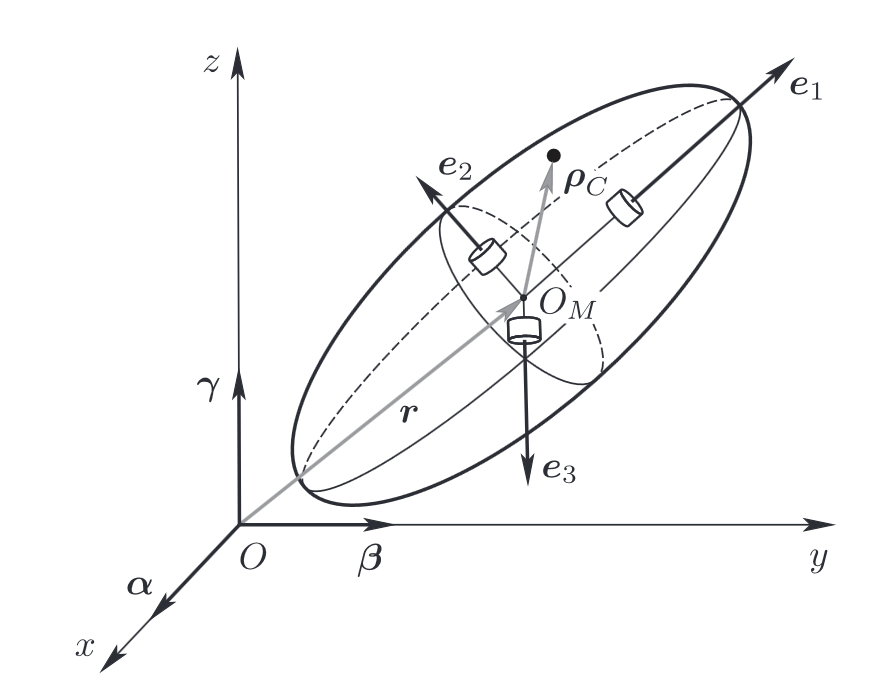
\includegraphics[width=0.5\linewidth]{BPR_Scheme.png}
		\caption{Схематическая модель безвинтового подводного робота с внутренними роторами, где $Oxyz$ -- неподвижная система координат, $O_M e_1 e_2 e_3$ -- подвижная система координат, $O_M$ -- геометрический центр эллипсоида, $\br$ -- радиус-вектор объекта, $\bbs \rho_C$ -- вектор центра масс системы в подвижной системе координат} \label{rotors}
	\end{center}
\end{figure}


Будем полагать, что конструкция удовлетворяет ряду условий:
\begin{enumerate}
	\item Оболочка является однородной, положение ее центра масс совпадает с геометрическим центром оболочки.
	\item В общем случае центр масс всей системы находится не в геометрическом центре оболочки;
	\item Все роторы одинаковы, осесимметричны и оси вращения  совпадают с их осями симметрии, то есть вращение роторов не изменяет распределение масс системы;
	%\item Ось вращения одного из роторов совпадает с осью винтовой симметрии оболочки;
	\item Оси вращения роторов взаимно перпендикулярны, а их угловые скорости являются заданными функциями времени $\omega _k \bigl( t \bigr),~k=1,2,3$.
\end{enumerate}

Выберем подвижную систему координат $O_M e_1 e_2 e_3$, жестко связанную с оболочкой, так что оси совпадают с главными осями инерции оболочки. Обозначим через $\bV$ и ${\bOm}$ скорость центра оболочки и его угловую скорость (все векторы, если не оговорено обратное, проецируются на подвижные оси).

Определим дополнительно неподвижную систему координат $O x y z$ и обозначим $\br = \bigl( x,\, y,\, z \bigr)$ -- координаты геометрического центра оболочки в этих осях. Обозначим также через ${\bal}$, ${\bbe}$, ${\bga}$ орты неподвижных осей $O x y z$, спроецированные на подвижные оси $e_1$, $e_2$, $e_3$, тогда ортогональная матрица
\begin{gather}
\bbQ =\begin{pmatrix}
\alpha _1 & \beta _1 & \gamma _1\\
\alpha _2 & \beta _2 & \gamma _2\\
\alpha _3 & \beta _3 & \gamma _3
\end{pmatrix} \in SO(3)
\label{eq.Qabg}
\end{gather}
характеризует ориентацию тела, а пара $\left( \br,\, \bm{Q} \right)$ однозначно определяет конфигурацию системы. Таким образом, конфигурационное пространство системы шестимерно и представляет собой $\mathbb{R}^3 \times SO(3)$.

Представление матрицы $\bbQ$ в форме \eqref{eq.Qabg} удобно при численных расчетах и построении явных управлений, обеспечивающих, например, вращение тела вокруг некоторого направления. Для проверки критерия управляемости Рашевского-Чжоу \cite{Rashevskyi_1938} более удобной является параметризация матрицы $\bbQ$ через углы Эйлера
{\small 
\begin{gather}
\bbQ = \begin{pmatrix}
\cos\psi \cos\varphi - \sin\psi\cos\theta\sin\varphi & \sin\psi \cos\varphi + \cos\psi \cos\theta \sin\varphi & \sin\theta \sin\varphi \\
-\cos\psi \sin\varphi - \sin\psi \cos\theta \cos\varphi & - \sin\psi \sin\varphi + \cos\psi \cos\theta \cos\varphi & \sin\theta \cos\varphi \\
\sin\psi \sin\theta & - \cos\psi \sin\theta & \cos\theta
\end{pmatrix},\label{eq.QEuler}
\end{gather}
}
где $\psi$ -- угол прецессии, $\theta$ -- угол нутации, $\varphi$ -- угол собственного вращения.


Эволюция углов Эйлера во времени описывается следующими уравнениями:
\begin{gather}
\begin{pmatrix}
\dot{\psi} \\ \dot{\theta} \\ \dot{\varphi}
\end{pmatrix} = \bPi \bOm,\quad \bPi = \begin{pmatrix}
\sin\varphi / \sin\theta & \cos\varphi / \sin\theta & 0 \\
\cos\varphi & -\sin\varphi & 0 \\
-\cot\theta \sin\varphi & -\cot\theta\cos\varphi & 1
\end{pmatrix}.\label{eq.Euler}
\end{gather}

Обозначим через $m_s$ -- массу оболочки, ${\bm I}_s$ -- ее центральный тензор инерции, $\bLam = \diag(\bLam_1, \bLam_2) $
%\begin{gather}
%\bLam = \begin{pmatrix}
%\bLam _1 & 0 \\
%0 & \bLam _2
%\end{pmatrix}\nonumber
%\end{gather}
-- матрицу коэффициентов присоединенных масс в системе $O_M e_1 e_2 e_3$, где $\bLam_1$ -- тензор присоединенных масс, $\bLam_2$ -- тензор присоединенных моментов инерции. Отметим, что в силу выбранных систем координат, тензоры $\bLam_1$ и $\bLam_2$ имеют диагональный вид: $\bLam_1=\diag(\lambda_1, \lambda_2, \lambda_3)$, $\bLam_2=\diag(\lambda_4, \lambda_5, \lambda_6)$. Тогда выражение для кинетической энергии оболочки примет вид
\begin{gather}
T_s = \frac{1}{2} m_s  \bigl( \bV,\, \bV \bigr) + \frac{1}{2} \bigl( {\bm I}_s {\bOm},\, {\bOm} \bigr),\nonumber
\end{gather}
а выражение кинетической энергии жидкости
\begin{gather}
T_f = \frac{1}{2} \bigl( \bLam_1 \bV,\, \bV \bigr) + \frac{1}{2} \bigl( {\bLam} _2 {\bOm},\, {\bOm} \bigr).\nonumber
\end{gather}

Обозначим через $m_R$ -- массу ротора, ${\bbI}_k$ -- центральный тензор инерции $k$-го ротора, записанный в системе координат $O_M e_1 e_2 e_3$, $\bn_k$ -- орт оси вращения $k$-го ротора неподвижный в системе $O_M e_1 e_2 e_3$, $\br_k$ -- радиус-вектор центра масс $k$-го ротора неподвижный в системе $O_M e_1 e_2 e_3$. Тогда кинетическая энергия $k$-го ротора примет вид
\begin{gather}
T_k = \frac{1}{2} m_R \bigl( \bV + {\bOm} \times \br_k, \bV + {\bOm} \times \br_k \bigr) + \frac{1}{2}\Bigl({\bm I}_k \bigl( {\bOm} + \omega_k \bn_k \bigr), {\bOm} + \omega_k \bn_k \Bigr).\nonumber
\end{gather}

Суммарная кинетическая энергия всей системы с учетом того, что оси роторов задаются собственными векторами их тензоров инерции, то есть ${\bbI}_k \bn_k = i_k \bn_k$, примет вид
\begin{gather}
\label{kinetic_energy}
\begin{split}
T = & T_f + T_s + \sum _{k=1}^3 T_k = \\
= & \frac{1}{2} \bigl( {\bbI} {\bOm},\, {\bOm} \bigr) + \bigl( {\bbB} {\bOm},\, \bV \bigr) + \frac{1}{2} \bigl( {\bbC} \bV,\, \bV \bigr) + \bigl( {\bOm},\, \bK(t) \bigr) + \frac{1}{2} \sum_{k=1}^3 i_k \omega_k^2 (t),
\end{split} \\
\bK(t)=\sum \limits_{k=0}^3 i_k \omega_k (t)\bn_k,
\label{eqK}
\end{gather}
где $\bbI$ --- тензор инерции всей системы вычисленный относительно геометрического центра оболочки, матрицы $\bbB$ и $\bbC$ зависят от распределения масс и формы оболочки, $\bK(t)$ --- вектор гиростатического момента. Матрицы $\bbI$, $\bbB$, $\bbC$ имеют вид
\begin{gather}
{\bbI} = {\bLam}_2 + {\bbI}_s + \sum _{k=1}^3 {\bbI}_k + \frac{1}{2} m_R \sum _{k=1}^3 \bigl( \br_k^2{\bbE} - \br_k \otimes \br_k \bigr),\nonumber \\
{\bbC} = m {\bbE} + {\bLam}_1 = \diag(c_1, \, c_2, \, c_3),\nonumber \\
{\bbB} = m \begin{pmatrix}\nonumber
0 & z_c & -y_c\\
-z_c & 0 & x_c\\
y_c & -x_c & 0
\end{pmatrix},\nonumber \\
m = m_s + 3 m_R,\nonumber
\end{gather}
где $x_c$, $y_c$, $z_c$ --- компоненты радиус-вектора $\bbs \rho_C$ центра масс системы.

%\begin{small}
	{\textbf{ Замечание.} Общее число параметров матриц $\bbC$, $\bbB$, $\bbI$ равно 21. С помощью подходящего выбора точки $O_M$ и ориентации осей $O_M e_1 e_2 e_3$ матрицу $\bbI$ можно привести к диагональному виду, $\bbB$ -- к симметрическому, а общее число параметров будет равно 15 \cite{Borisov_Mamaev}. Исследования, которые будут проводиться в дальнейшем, будут осуществляться численно, поэтому вопрос о количестве параметров не является принципиальным.}
%\end{small}

Уравнения движения рассматриваемой системы имеют вид классических уравнений Кирхгофа \cite{Borisov_Mamaev}
\begin{gather}
\label{Kirchhoff}
\frac{d}{dt} \biggl( \frac{\partial T}{\partial \bV} \biggr) + {\bOm} \times \frac{\partial T}{\partial \bV}=0, \quad \frac{d}{dt}\biggl( \frac{\partial T}{\partial {\bOm}} \biggr) + {\bOm} \times \frac{\partial T}{\partial {\bOm}} + \bV \times \frac{\partial T}{\partial \bV} = 0 \nonumber
\end{gather}
и с учетом (\ref{kinetic_energy}) могут быть записаны в виде
\begin{gather}
\label{motion_eq}
\begin{split}
{\bbC} \dot{\bV} + {\bbB} \dot{{\bOm}} = & \bigl( {\bbC} \bV + {\bbB} {\bOm} \bigr) \times {\bOm},\\
{\bbB}^T \dot{\bV} + {\bbI} \dot{{\bOm}} + \dot{\bK}(t) = & \bigl( {\bbB}^T \bV + {\bbI} {\bOm} + \bK(t) \bigr) \times {\bOm} + \bigl( {\bbC} \bV + {\bbB} {\bOm} \bigr) \times \bV = 0.
\end{split}
\end{gather}

Данные уравнения необходимо дополнить уравнениями эволюции переменных $\bigl( \br,\, {\bbQ} \bigr)$, которые описываются уравнениями Пуассона и кинематическими соотношениями следующего вида
\begin{gather}
\label{kinematics_abg}
\dot{{\bal}} = {\bal} \times {\bOm},\quad \dot{{\bbe}} = {\bbe} \times {\bOm},\quad \dot{{\bga}} = {\bga} \times {\bOm},\\
\dot{\br} = {\bbQ}^T \bV.
\label{kinematics_r}
\end{gather}

Уравнения \eqref{motion_eq}, \eqref{kinematics_abg}, \eqref{kinematics_r} полностью описывают движение рассматриваемой системы. Однако удобней записать данные уравнения в гамильтоновой форме \cite{Clebsch}:
\begin{gather}
\label{motion_ham}
\dot{\bP}= \bP \times {\bOm},\,\dot{\bM} = \bM \times {\bOm} + \bP \times \bV,
\end{gather}
где $\bP = \dfrac{\partial T}{\partial \bV}$ и $\bM = \dfrac{\partial T}{\partial {\bOm}}$ имеют гидродинамический смысл и называются, соответственно, импульсивным моментом и импульсивной силой~\cite{Borisov_Mamaev}. При этом $\bV$ и ${\bOm}$ связаны с этими векторами следующим образом:
\begin{gather}
\label{p_and_M}
\begin{split}
\bP = & {\bbC} \bV + {\bbB} {\bOm},\, \bM = {\bbB}^T \bV + {\bbI} {\bOm} + \bK(t),\\
\bV = & {\bbC}^{-1} \bigl( \bP - {\bbB} {\bOm} \bigr),\, {\bOm} = \bigl({\bbI} - {\bbB}^T {\bbC}^{-1} {\bbB} \bigr)^{-1} \bigl( \bM - \bK(t) - {\bbB}^T {\bbC}^{-1} \bP \bigr).
\end{split}\nonumber
\end{gather}

%Уравнения \eqref{motion_ham} являются гамильтоновыми на алгебре $e(3)$ с гамильтонианом
%\begin{gather}
%H = \bigl( \bM,\, {\bOm} \bigr) - T \big| _{{\bOm},\, \bV \rightarrow \bM,\, \bP}\nonumber
%\end{gather}

Уравнения \eqref{kinematics_abg} допускают шесть геометрических интегралов движения:
\begin{gather}
{\bal}^2={\bbe}^2={\bga}^2=1,\, \bigl({\bal},\, {\bbe} \bigr) = \bigl({\bal},\, {\bga} \bigr) = \bigl({\bbe},\, {\bga} \bigr) = 0.\nonumber
\end{gather}

Как указано в \cite{Kozlov_Ramodanov_PMM_2001} уравнения (\ref{motion_ham}) допускают еще шесть первых интегралов движения:
\begin{gather}
(\bP,\, {\bal}),\, (\bP,\, {\bbe}),\, (\bP,\, {\bga}),\, (\bM + \br \times \bP,\, {\bal}),\, (\bM + \br \times \bP,\, {\bbe}),\, (\bM + \br \times \bP,\, {\bga}) \label{integrals}
\end{gather}

Данные интегралы движения имеют следующий смысл: при движении тела в идеальной жидкости векторы $\bP$ и $\bM + \br \times \bP$ сохраняются в абсолютном пространстве. В случае движения из состояния покоя первые интегралы \eqref{integrals} приобретают особенно простой вид:
\begin{gather}
\bP = 0, \quad \bM = 0, \nonumber
\end{gather}
а выражения для скоростей можно записать как
\begin{gather}
\bV = - \bbC^{-1} \bbB \bOm, \label{v} \nonumber \\
\bOm = - \bigl(\bbI - \bbB^T \bbC^{-1} \bbB \bigr)^{-1} \bK(t). \label{omega} 
\end{gather}
%\textit{Замечание}. Выражения (\ref{p_and_M}) показывают, что для уравновешенной механической системы (центр масс совпадает с геометрическим центром оболочки)
%
%если механическая система уравновешена, то есть центр масс совпадает с геометрическим центром оболочки, матрица ${\bbB}$ становится нулевой, то перемещение в идеальной жидкости невозможно.

Таким образом при движении из состояния покоя система уравнений описывающих эволюцию ориентации и траектории движения при заданном управлении имет вид:

\begin{gather}
\begin{gathered}
\dot{{\bal}} = {\widetilde{\bbI} \bK(t)}  \times {\bal},\\
\dot{{\bbe}} = {\widetilde{\bbI} \bK(t)}  \times {\bbe},\\
\dot{{\bga}} = {\widetilde{\bbI} \bK(t)}  \times {\bga},\\
\dot{\br} =  {\bbQ}^T \bbC^{-1} \bbB \widetilde{\bbI} \bK(t),
\end{gathered}
\label{motion_eq_simple}
\end{gather}
где $\widetilde{\bbI} = \bigl(\bbI - \bbB^T \bbC^{-1} \bbB \bigr)^{-1}$.

В системе уравнений~\eqref{motion_eq_simple} вектор гиростатического момента $ \bK(t) $ является управляющим воздействием, так как зависит от угловых скоростей роторов: $ \bK(t)=\sum \limits_{k=0}^3 i_k \omega_k (t)\bn_k $.

Решения системы уравнений \eqref{motion_eq_simple} относительно $\bK(t)$ позволяют находить управляющие воздействия $\omega_k (t)$ для движения вдоль заданной траектории. %, которая описывается уравнением \eqref{kinematics_r}.


\section{Исследование уравнений движения}

В качестве исследований уравнений движения сначала проверим возможность управления системы на нулевом уровне первых интегралов с помощью теоремы Рашевского-Чжоу. Далее рассчитаем теоретические траектории движения при различных управляющих воздействиях.

\subsection{Исследование управляемости}

Для исследования управляемости представим систему уравнений движения в виде
\begin{gather}
\dot{\bq} = \begin{pmatrix}
\bbQ^T\bbC^{-1} \bbB \\ - \bPi
\end{pmatrix} \widetilde{\bbI} \bK(t),\label{eq.onLevel0}
\end{gather}
где $\bq = (x,\, y,\, z \, \psi,\, \theta,\, \varphi)$ -- вектор, определяющий положение тела.% в конфигурационном пространстве $\mathcal{G}$. 
Таким образом, на нулевом уровне интегралов движения, исследование управляемости сводится к изучению уравнений \eqref{eq.onLevel0}, описывающих эволюцию только конфигурационных переменных, исключая из рассмотрения динамические переменные.

Поскольку матрица $\widetilde{\bbI}$ невырожденная, то с помощью \eqref{omega} от управлений собственным гиростатическим моментом можно перейти к управлению угловыми скоростями оболочки $\bOm = (\Omega_1,\, \Omega_2,\, \Omega_3)$, а уравнения \eqref{eq.onLevel0} записать в следующей форме
{\small \begin{gather}
\dot{\bq} = \bX_1 (\psi,\, \theta,\, \varphi) \Omega_1 + \bX_2 (\psi,\, \theta,\, \varphi) \Omega_2 + \bX_3 (\psi,\, \theta,\, \varphi) \Omega_3,\label{eq.zu123}\\
\begin{gathered}
\bX_1 = \left( \dfrac{\sin \varphi}{\sin \theta} ,\, \cos \varphi ,\, -\cot\theta \sin\varphi ,\, 
\dfrac{ m y_c\alpha_3 }{c_3} - \dfrac{m z_c \alpha_2}{c_2}, \, 
\dfrac{m y_c \beta_3 }{c_3} - \dfrac{m z_c \beta_2}{c_2} ,\, 
\dfrac{m y_c \gamma_3 }{c_3} - \dfrac{m z_c \gamma_2}{c_2} \right)^T,\\
\bX_2 = \left( \dfrac{\cos \varphi}{\sin \theta} ,\, -\sin \varphi ,\, -\cot\theta \cos\varphi ,\, 
\dfrac{m z_c\alpha_1 }{c_1} - \dfrac{m x_c \alpha_3}{c_3}, \, 
\dfrac{m z_c \beta_1 }{c_1} - \dfrac{m x_c \beta_3}{c_3} ,\, 
\dfrac{m z_c \gamma_1 }{c_1} - \dfrac{m x_c \gamma_3}{c_3} \right)^T,\\
\bX_3 = \left( 0 ,\, 0 ,\, 1 ,\, 
\dfrac{m x_c \alpha_2 }{c_2} - \dfrac{m y_c \alpha_1}{c_1}, \, 
\dfrac{m x_c \beta_2 }{c_2} - \dfrac{m y_c \beta_1}{c_1} ,\, 
\dfrac{m x_c \gamma_2 }{c_2} - \dfrac{m y_c \gamma_1}{c_1} \right)^T,
\end{gathered}\label{eq.com0_Lam0noG}
\end{gather}}
где $\alpha_i$, $\beta_i$, $\gamma_i$ выражаются через углы Эйлера с помощью соотношений \eqref{eq.Qabg}, \eqref{eq.QEuler}.

Согласно теореме Рашевского-Чжоу \cite{Rashevskyi_1938} система вида $\dot{\bq} = \sum_{i=1}^{M}\bX_i(\bq) u_i$, управляема в некоторой области $N$-мерного пространства, если среди векторных полей $\bX_i$ и всевозможных их коммутаторов $\bX_{i,j} = [\bX_i,\, \bX_j]$, $\bX_{k,(i,j)} = [\bX_k,\, \bX_{i,j}]$, \ldots, составленных последовательными применениями скобки Ли $[\cdot,\, \cdot]$, найдется $N$ линейно независимых в каждой точке области.

Скобка Ли для векторных полей $ \bbs v $ и $ \bbs u $ имеет выражение
\begin{gather}
[\bbs v, \bbs u]_{i}=\sum_{j}v_{j}\frac{\partial u_{i}}{\partial x_{j}}-u_{j}\frac{\partial v_{i}}{\partial x_{j}},
\end{gather}
где $ x_{j} $ -- компоненты вектора обобщенных координат.

Если, в данном случае для 6-мерного пространства состояний, определитель матрицы, составленной из компонент шести векторных полей, не равен нулю, то данные векторные поля линейно независимые.

Построим следующие векторные поля:
\begin{gather}
\begin{gathered}
\bX_{1,2} = \left[ \bX_1,\, \bX_2\right],\quad \bX_{3,1} = \left[ \bX_3,\, \bX_1\right],\quad \bX_{2,3} = \left[ \bX_2,\, \bX_3\right], \\  
\bX_{1,(2,3)} = \left[ \bX_1,\, \bX_{2,3}\right],\quad \bX_{2,(3,1)} = \left[ \bX_2,\, \bX_{3,1}\right], \quad \bX_{3,(1,2)} = \left[ \bX_3,\, \bX_{1,2}\right].\\
\end{gathered}\label{eq.fieldsDeficit}
\end{gather}
Выберем из (\ref{eq.com0_Lam0noG}) и (\ref{eq.fieldsDeficit}) три набора векторных полей
\begin{gather*}
\begin{gathered}
\Bigl( \bX_1,\, \bX_2,\,\bX_3,\,\bX_{1,2},\,\bX_{2,3},\,\bX_{2,(3,1)},\, \Bigr),\quad
\Bigl( \bX_1,\, \bX_2,\,\bX_3,\,\bX_{2,3},\,\bX_{3,1},\,\bX_{3,(1,2)},\, \Bigr), \\
\Bigl( \bX_1,\, \bX_2,\,\bX_3,\,\bX_{3,1},\,\bX_{1,2},\,\bX_{1,(2,3)},\, \Bigr).
\end{gathered}\label{eq.sets}
\end{gather*}

%Определитель матрицы:
%\begin{gather*}
%\begin{gathered}
%\det\Bigl( \bX_1,\, \bX_2,\,\bX_3,\,\bX_{1,2},\,\bX_{2,3},\,\bX_{3,1}\, \Bigr) = 
% {\frac {2{m}^{3}{x_c}\,{ y_c}\,{ z_c}\, \left( {c_2}
%		-{ c_3} \right)  \left( -{ c_3}+{c_1} \right)  \left( {c_1}-
%		{c_2} \right) }{{{c_3}}^{2}{{c_2}}^{2}{{c_1}}^{2}\sin
%		\left( \theta \right) }}
%\end{gathered}\label{det1}
%\end{gather*}
%
%Данный определитель обращается в 0 при выполнении одного из условий:
%\begin{gather}
%\begin{gathered}
%x_c = 0,\ 
%y_c = 0, \
%z_c = 0, \
%(c_2 - c_3) = 0,\
%(-c_3+c_1) = 0, \
%(c_1-c_2) = 0.
%\end{gathered}\label{if}
%\end{gather}

Условия линейной зависимости векторных полей в указанных наборах имеют вид
\begin{gather}
\begin{gathered}
x_c(c_2 - c_3) = 0,\quad
y_c(c_3-c_1) = 0, \quad
z_c(c_1-c_2) = 0.
\end{gathered}\label{eq.lin}
\end{gather}

Из (\ref{eq.lin}) следует, что среди полей (\ref{eq.com0_Lam0noG}), (\ref{eq.fieldsDeficit}) всегда можно выбрать шесть линейно независимых векторных полей за исключением случаев одновременного выполнения всех трех равенств (\ref{eq.lin}). Отметим, что уравнения (\ref{eq.lin}) зависят только от параметров задачи, т.е. накладывают ограничения на конструкцию рассматриваемой системы.

Таким образом, движение в идеальной жидкости однородной оболочки, имеющей форму эллипсоида, вполне управляемо с помощью вращения трех роторов, за исключением трех частных случаев:
\begin{enumerate}
	\item Система “ оболочка + роторы” уравновешена;
	\item Оболочка имеет сферическую форму;
	\item Оболочка имеет форму эллипсоида вращения, а центра масс всей системы	расположен на оси вращения.
\end{enumerate}

Таким образом, чтобы получить управляемый объект с формой оболочки в виде эллипсоида вращения с центром масс всей системы в геометрическом центре эллипсоида, необходимо внести асимметрию в форму. Это можно сделать добавив к оболочке винтовые лопасти. Так, объект будет представлять из себя трехлопастной винт. 

Получить уравнения движения для трехлопастного винта можно, используя вывод, описанный в разделе \ref{sec:ch2/sec1}. Отличие будет в матрице коэффициентов присоединенных масс 
\begin{gather}
\bLam = \begin{pmatrix}
\bLam _1 & \bLam_{12} \\
\bLam_{12}^{T} & \bLam _2
\end{pmatrix}\nonumber,
\end{gather}
где $\bLam_{12}$ -- тензор, возникающий вследствие винтовой симметрии. А матрица $ \bbB $ будет иметь вид
\begin{gather*}
{\bbB} = \bLam_{12} + m \begin{pmatrix}
0 & z_c & -y_c\\
-z_c & 0 & x_c\\
y_c & -x_c & 0
\end{pmatrix}. 
\end{gather*}
В случае совпадения центра масс системы и геометрического центра эллипсоида матрица $ \bbB $ примет диагональный вид.

Учитывая вышеописанные дополнения к математической модели, для описания движения можно использовать уравнения (\ref{motion_eq_simple}).

Исследования управляемости системы в виде трехлопастного винта показывают, что определитель матрицы $ \Bigl( \bX_1,\, \bX_2,\,\bX_3,\,\bX_{1,2},\,\bX_{2,3},\,\bX_{3,1}\, \Bigr) $ не равен нулю в каждой точке конфигурационного пространства, что доказывает, что данная система вполне управляема.

\subsection{Коэффициенты и параметры модели}

Для объекта, имеющего форму эллипсоида вращения, значения тензоров присоединенных масс и присоединенных моментов инерции можно рассчитать используя справочные материалы~\cite{Korotkin}.

Для винтового тела, с конструкцией, описанной в главе~\ref{ch:ch3}, коэффициенты присоединенных масс определяются интегрированием по поверхности тела $\Sigma$:
\begin{gather}
\lambda _{ik} = \rho \int _\Sigma \varphi _i \frac{\partial \varphi _k}{\partial n} d \sigma,
\end{gather}
где потенциалы $\varphi _i, \quad i = \overline{1,6}$ находятся из численного решения шести задач Неймана
\begin{gather}
\Laplace \varphi _i = 0 \label{lapl}
\end{gather}
с граничными условиями на бесконечности
\begin{gather}
\nabla \varphi _i = 0
\end{gather}
и на границе твердого тела
\begin{gather}
\frac{\partial \varphi _i}{\partial n} = n_i, \quad \frac{\partial \varphi _{i+3}}{\partial n} = (\br \times \bn) _i, \quad i = \overline{1,3}.
\end{gather}

Уравнения \eqref{lapl} решались методом конечных объемов на тетраэдрических сетках.

Моменты инерции объекта можно вычислить в программном продукте SolidWorks, разработав твердотельные модели всех элементов конструкции, учитывая плотность материалов, из которых они изготовлены.

Для безвинтового подводного робота с внутренними роторами с конструкцией и размерами, описанными в следующей главе, запишем параметры, определяемые конструкцией: тензор присоединенных масс, тензор присоединенных моментов инерции, тензор, возникающий вследствие винтовой симметрии; тензор инерции оболочки, тензоры инерции роторов; радиус-векторы центра масс роторов. Все параметры имеют размерность в соответствии с системой СИ.

{\small \begin{gather*}
\begin{gathered}
%\bLam_1 = diag(3.3306; 4.667; 4.667); \qquad 
%\bLam_2 = diag(0.0134; 0.0107; 0.0107);
\bLam_1 =\begin{pmatrix}
3.330606 	& 0	 		& 0\\
0 			& 4.666924	& 0\\
0 			& 0			& 4.666924
\end{pmatrix}, 
\quad 
\bLam_2 =\begin{pmatrix}
0.013439	& 0	 		& 0\\
0 			& 0.010745 	& 0\\
0 			& 0			& 0.010745
\end{pmatrix}, 
\\
\bLam_{12} =\begin{pmatrix}
-0.138752	& 0	 		& 0\\
0 			& 0.069489 	& 0\\
0 			& 0			& 0.069489
\end{pmatrix}, 
\quad 
{\bm I}_s =\begin{pmatrix}
0.006424 	& 0	 		& 0\\
0 			& 0.012909	& 0\\
0 			& 0			& 0.012909
\end{pmatrix}, 
\\
{\bm I}_1 =\begin{pmatrix}
0.001493	& 0	 		& 0\\
0 			& 0.000778 	& 0\\
0 			& 0			& 0.000778
\end{pmatrix}, 
\quad 
{\bm I}_2 =\begin{pmatrix}
0.000274 	& 0	 		& 0\\
0 			& 0.000522	& 0\\
0 			& 0			& 0.000247
\end{pmatrix}, 
\\
{\bm I}_3 =\begin{pmatrix}
0.000274	& 0	 		& 0\\
0 			& 0.000274 	& 0\\
0 			& 0			& 0.000522
\end{pmatrix}, 
\\
\br_1 = (0.08318; 0; 0), \quad
\br_2 = (0; 0.06135; 0), \quad
\br_3 = (0; 0; 0.06135).
\end{gathered}
\label{ParamBPR}
\end{gather*}}

В дальнейшем данные значения коэффициентов будут использованы для расчета теоретических траекторий движения используя разработанную математическую модель.

% ${\bm I}_s = diag(0.006424; 0.012909; 0.012909)$.
%Тензоры инерции роторов: ${\bm I}_1 = diag(0.001493; 0.000778; 0.000778)$. ${\bm I}_2 = diag(0.000274; 0.000522; 0.000247)$. ${\bm I}_3 = diag(0.000274; 0.000274; 0.000522)$.

%Радиус векторы центра масс роторов: $\br_1 = (0.08318; 0; 0)$, $\br_2 = (0; 0.06135; 0)$, $\br_1 = (0; 0; 0.06135)$,

\subsection{Моделирование теоретических траекторий}\label{ch2_sec_Modelling}

Наиболее простым видом движения робота является движение при вращении внутренних роторов с постоянной скоростью. Рассмотрим движение тела при постоянных скоростях вращения роторов $\bbs\omega = (\omega_1, \omega_2, \omega_3)^T$. 

Все расчеты траектории движения проводились со следующими начальными условиями:
\begin{gather*}
\begin{gathered}
\bal(0) =  \begin{pmatrix}
1 \\ 0 \\ 0
\end{pmatrix}, \quad
\bbe(0) =  \begin{pmatrix}
0 \\ 1 \\ 0
\end{pmatrix}, \quad
\bga(0) =  \begin{pmatrix}
0 \\ 0 \\ 1
\end{pmatrix}, \\
x(0)=0, \quad y(0)=0, \quad z(0)=0.
\end{gathered}
\end{gather*}

Проведем моделирование при $\omega_1=10$ рад/с, $\omega_2=0$, $\omega_3=0$. Тело продвинулось вдоль оси $X$ на расстояние 0.0575 метра. Результат моделирования в виде траектории движения представлен на рисунке~\ref{ModelTrBPR}а.

Проведем моделирование при $\omega_1=0$, $\omega_2=10$ рад/с, $\omega_3=0$. Тело продвинулось вдоль оси $Y$ на расстояние 0.0066 метра. Результат моделирования в виде траектории движения представлен на рисунке~\ref{ModelTrBPR}б.

Проведем моделирование при $\omega_1=0$, $\omega_2=0, \omega_3=10$ рад/с. Тело продвинулось вдоль оси $Z$ на расстояние 0.0066 метра. Результат моделирования в виде траектории движения представлен на рисунке~\ref{ModelTrBPR}в.

\begin{figure}[!ht]
	\begin{minipage}[h]{0.3\linewidth}
		\center{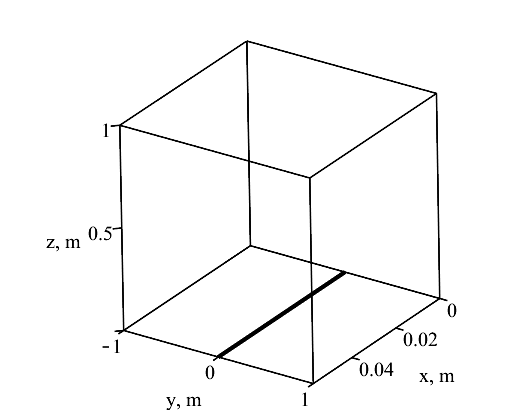
\includegraphics[width=0.9\linewidth]{ModelTrBPR1_.png} }
	\end{minipage}
	\hfill
	\begin{minipage}[h]{0.3\linewidth}
		\center{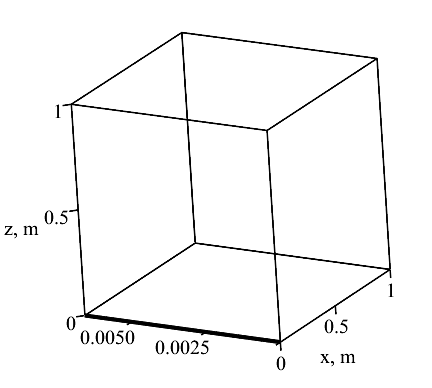
\includegraphics[width=0.9\linewidth]{ModelTrBPR2_.png} }
	\end{minipage}
	\hfill
	\begin{minipage}[h]{0.3\linewidth}
		\center{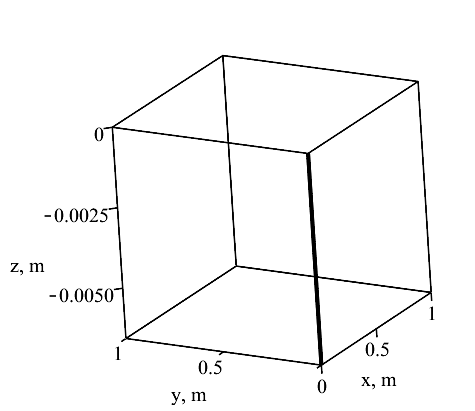
\includegraphics[width=1\linewidth]{ModelTrBPR3_.png} }
	\end{minipage}

	\begin{minipage}[h]{0.3\linewidth}
		\center{а}
	\end{minipage}
	\hfill
	\begin{minipage}[h]{0.3\linewidth}
		\center{б}
	\end{minipage}
	\hfill
	\begin{minipage}[h]{0.3\linewidth}
		\center{в}
	\end{minipage}
	
	\caption{Расчетная траектория движения для а)$\omega_1=10$ рад/с, $\omega_2=0$, $\omega_3=0$; б)$\omega_1=0$, $\omega_2=10$ рад/с, $\omega_3=0$; в)$\omega_1=0$, $\omega_2=0, \omega_3=10$. Время моделирования -- 3 секунды.}
	\label{ModelTrBPR}
\end{figure}

Как видно из графиков, при вращении одного ротора с постоянной угловой скоростью, робот движется по прямолинейной траектории. При вращении малых роторов результат отличается только направлением движения, так как тело обладает динамической симметрией. Движение происходит вдоль оси, на которой расположен ротор.

Проведем моделирование при $\omega_1=10$ рад/с, $\omega_2=10$ рад/с, $\omega_3=0$. Результат моделирования в виде траектории движения представлен на рисунке~\ref{ModelTrBPR12}.

\begin{figure}[h]
	\centering
	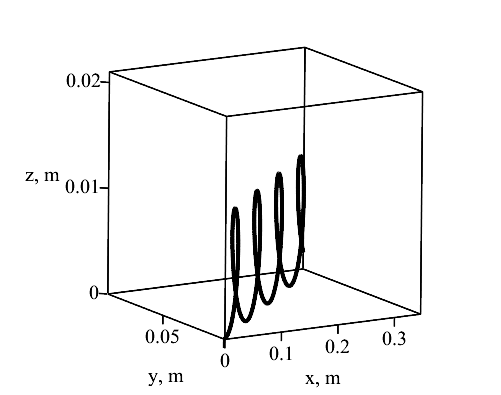
\includegraphics[width=0.4\linewidth]{ModelTrBPR12_.png}%
	\caption{Расчетная траектория движения для $\omega_1=10$ рад/с, $\omega_2=10$ рад/с, $\omega_3=0$. Время моделирования -- 5 секунд.}
	\label{ModelTrBPR12}
\end{figure}

При вращении большого и одного малого ротора одновременно с постоянной угловой скоростью тело движется по траектории в виде спирали, а ось спирали параллельна плоскости $OXY$. Пропорциональное увеличение скоростей вращения роторов приведет только к более быстрому продвижению по спирали. Следует отметить, что при вращении второго малого ротора в связке с большим, траектория движения будет аналогичной, изменится направление движения. Движение происходит в направлении вектора $\bK$.

Проведем моделирование при $\omega_1=0$, $\omega_2=10$ рад/с, $\omega_3=10$ рад/с. Результат моделирования в виде траектории движения представлен на рисунке~\ref{ModelTrBPR23}. Тело продвинулось в плоскости $OYZ$ на расстояние 0.0619 метра.

\begin{figure}[h]
	\centering
	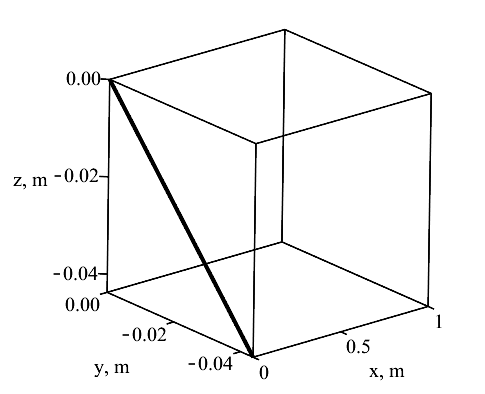
\includegraphics[width=0.4\linewidth]{ModelTrBPR23.png}%
	\caption{Расчетная траектория движения для $\omega_1=0$, $\omega_2=10$ рад/с, $\omega_3=10$ рад/с. Время моделирования -- 5 секунд.}
	\label{ModelTrBPR23}
\end{figure}

Проведем моделирование при $\omega_1=10$ рад/с, $\omega_2=10$ рад/с, $\omega_3=10$ рад/с. Результат моделирования в виде траектории движения представлен на рисунке~\ref{ModelTrBPR123}. Тело движется по траектории в виде спирали, однако, в сравнении с расчетами, представленными на рисунке~\ref{ModelTrBPR12}, ось спирали расположена под некоторым углом к плоскости $OXY$.

\begin{figure}[h]
	\centering
	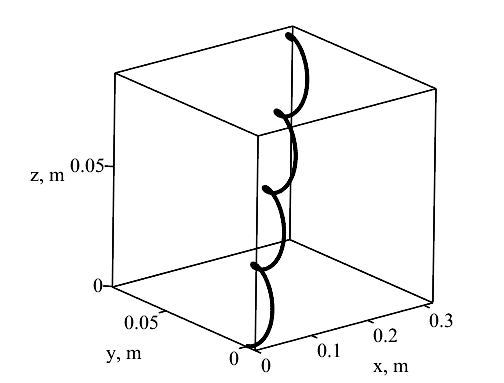
\includegraphics[width=0.4\linewidth]{ModelTrBPR123.png}%
	\caption{Расчетная траектория движения для $\omega_1=10$ рад/с, $\omega_2=10$ рад/с, $\omega_3=10$ рад/с. Время моделирования -- 5 секунд.}
	\label{ModelTrBPR123}
\end{figure}

Разработанная теоретическая модель движения показывает, что в рамках модели идеальной жидкости безвинтовой подводный робот с внутренними роторами движется с постоянной линейной и угловой скоростью при постоянной скорости вращения роторов. Изменяя значения угловых скоростей отдельного ротора, можно двигаться вдоль прямой в любом направлении.

\section{Выводы по главе}

В главе представлена математическая модель трехмерного движения безвинтового подводного робота с внутренними роторами, записанная в виде уравнений Кирхгоффа. Полученные уравнения исследованы на управляемость. Показано, для полной управляемости к объекту в виде эллипсоида вращения необходимо добавить винтовые лопасти. Расчитаны все входящие в модель коэффициенты для конкретной модели робота, проведены расчеты теоретических траекторий при различных управляющих воздействиях. Показано, что для движения робота в рамках модели идеальной жидкости с постоянной угловой и линейной скоростями, достаточно задавать постоянные скорости вращения роторов.
%\section{Разработка и оценка алгоритма управления}
%
%На основе предыдущих разделов определить управляющие воздействия.
%
%\todo{1. Примеры решения обратной задачи: задана траектория - получили моменты - угловые скорости - напряжения(токи) 
%	что-то похожее есть тут: \textit{Борисов А. В., Килин А. А., Мамаев И. С., Как управлять шаром Чаплыгина при помощи роторов, Нелинейная динамика, 2012, т. 8, № 2, с. 289-307 } в разделе 5}
%	
%	\todo{2. возможно с учетом технических ограничений ускорений и моментов (т.е. попытаться максимально возможные скорости реализовать и для них построить траектории)}
%	
%	\todo{3. выбор коэффициентов регулирования}

